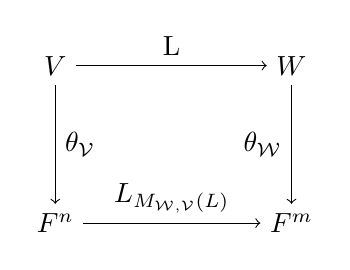
\begin{tikzpicture}
	\node (V) at (0,2) {$V$};
	\node (Fn) at (0,0) {$\mathbb{F}^n$};
	\node (W) at (3,2) {$W$};
	\node (Fm) at (3,0) {$\mathbb{F}^m$};

	\draw[->] (V) -- (Fn)  node[midway,right] {$\theta_\mathcal{V}$};
	\draw[->] (Fn) -- (Fm) node[midway,above] {$L_{M_{\mathcal{W},\mathcal{V}}(L)}$};
	\draw[->] (V) -- (W)   node[midway,above] {L};
	\draw[->] (W) -- (Fm)  node[midway,left] {$\theta_\mathcal{W}$};
\end{tikzpicture}
